\section{REFERENCIAL TEÓRICO}\label{sec:referencial}

\subsection{Panorama bibliométrico da literatura}\label{sec:bibliometria}

Para dimensionar o campo e orientar a seleção das referências, realizou-se um levantamento bibliométrico na base Scopus, processado com o pacote bibliometrix \citep{AriaCuccurullo2017}, em formato inspirado na abertura de \citet{Baker2022}. A busca, feita em 22 de outubro de 2026 nos títulos, resumos e palavras-chave, usou a expressão em inglês (\textit{``flypaper effect'' OR ``fiscal illusion'' OR ``intergovernmental transfer*'' OR ``intergovernmental grant*''}) AND (\textit{municipal* OR ``local government*'' OR subnational}) e foi restrita a artigos de periódicos publicados entre 2016 e 2026. Termos como \textit{fiscal transfers}, \textit{revenue sharing} e \textit{equalization} não foram incluídos; o conjunto recuperado é, portanto, uma amostra da literatura sobre transferências a governos locais, não o seu universo.

A busca retornou 327 artigos, dos quais 54 (16,5\%) tratam especificamente de efeito \textit{flypaper} ou de ilusão fiscal, critério aplicado aos títulos, resumos e palavras-chave (Tabela~\ref{tab:bibliometria} e Figura~\ref{fig:producao}). Considerados apenas os anos completos, a produção subiu de 23 artigos por ano em 2016--2019 para 32 em 2020--2022 e ficou em 29 em 2023--2025; somados, os períodos têm 92, 97 e 138 artigos, este último com 2026 incompleto. Os artigos específicos somam 15, 20 e 19 nesses períodos, ou 16,3\%, 20,6\% e 13,8\% do total. Com contagens tão pequenas, a variação dessas participações não permite afirmar uma mudança de agenda; indica apenas que os dois conceitos ocupam uma fatia estável e minoritária de uma literatura que cresceu até 2022 e depois se estabilizou.

A distribuição por periódico mostra onde esses conceitos circulam. Os títulos que mais publicam pertencem às finanças públicas e à economia política, com destaque para \textit{Local Government Studies} e \textit{Public Finance Review}, com 11 artigos cada. Em \textit{Local Government Studies} e \textit{Lex Localis}, cerca de metade dos artigos trata de \textit{flypaper} ou de ilusão fiscal; no \textit{European Journal of Political Economy}, nenhum dos dez artigos emprega esses termos, embora alguns tratem do fenômeno, como o de \citet{Shani2023}. Os demais 247 artigos (75,5\%) dispersam-se por outros periódicos. Essa base, complementada por estudos brasileiros não indexados na Scopus e por clássicos indispensáveis, forneceu o núcleo das referências discutidas a seguir.

\IfFileExists{tabelas/tabela1_bibliometria.tex}{\begin{table}[H]
\centering\footnotesize\setlength{\tabcolsep}{5pt}
\caption{Uso dos conceitos de efeito \textit{flypaper} e ilusão fiscal na literatura sobre transferências a governos locais, por periódico (2016--2026)}
\label{tab:bibliometria}
\begin{threeparttable}
\begin{tabular}{lccc}
\toprule
 & (1) & (2) & (3) \\
 & Transferências a & \textit{Flypaper} ou & (2)/(1) \\
Periódico & governos locais & ilusão fiscal & (\%) \\
\midrule
Local Government Studies & 11 & 6 & 54,5\% \\
Public Finance Review & 11 & 3 & 27,3\% \\
European Journal of Political Economy & 10 & 0 & 0,0\% \\
International Tax and Public Finance & 10 & 1 & 10,0\% \\
Public Choice & 8 & 2 & 25,0\% \\
Public Budgeting and Finance & 7 & 1 & 14,3\% \\
Lex Localis & 6 & 3 & 50,0\% \\
Regional Studies & 6 & 0 & 0,0\% \\
World Development & 6 & 0 & 0,0\% \\
Regional Science and Urban Economics & 5 & 1 & 20,0\% \\
Demais periódicos & 247 & 37 & 15,0\% \\
\midrule
Total & 327 & 54 & 16,5\% \\
\bottomrule
\end{tabular}
\begin{tablenotes}[flushleft]\footnotesize
\item Nota: A tabela resume o número de artigos publicados em periódicos científicos entre 2016 e 2026 sobre transferências intergovernamentais a governos locais. A busca foi realizada em 22/10/2026 na base Scopus, nos campos título, resumo e palavras-chave, com a expressão: ("flypaper effect" OR "fiscal illusion" OR "intergovernmental transfer*" OR "intergovernmental grant*") AND (municipal* OR "local government*" OR subnational), restrita a artigos de periódico publicados entre 2016 e 2026. A busca retornou 327 artigos. A coluna (1) apresenta todos os artigos; a coluna (2), os que tratam especificamente de efeito flypaper ou de ilusão fiscal (termos presentes no título, no resumo ou nas palavras-chave; artigos que tratam do fenômeno sem usar esses termos ficam apenas na coluna 1); a coluna (3), a participação de (2) em (1). As linhas listam os dez periódicos com mais artigos; os demais estão agregados. Os dados de 2026 são parciais (artigos indexados até a data da busca). Processamento: pacote bibliometrix (Aria e Cuccurullo, 2017) no R.
\end{tablenotes}
\end{threeparttable}
\end{table}
}{}

\IfFileExists{figuras/figura_producao_anual.png}{%
\begin{figure}[H]
  \centering
  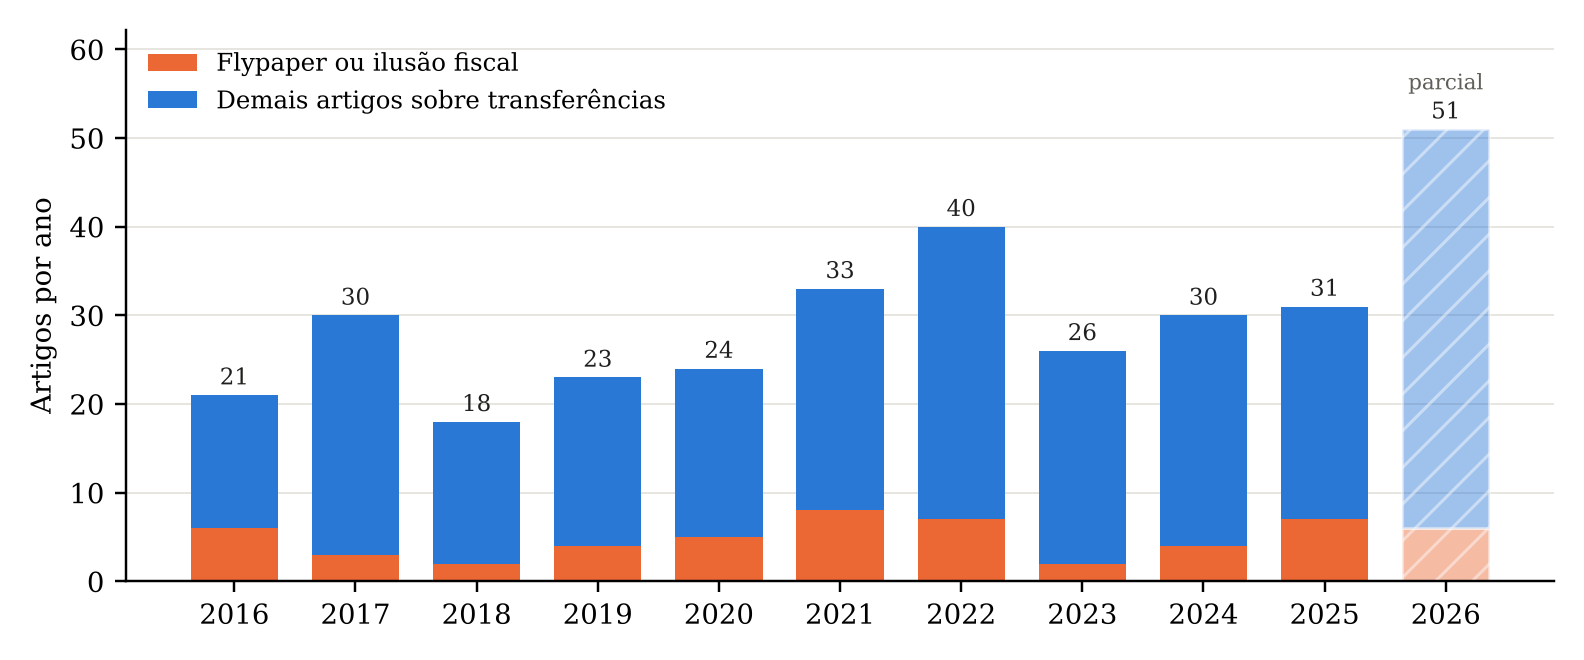
\includegraphics[width=0.9\textwidth]{figuras/figura_producao_anual.png}
  \caption{Produção anual de artigos recuperados pela busca (2016--2026): total e artigos sobre efeito \textit{flypaper} ou ilusão fiscal}
  \label{fig:producao}
  \fonte{elaboração própria a partir da base Scopus (busca em 22/10/2026), com a contagem do bibliometrix \citep{AriaCuccurullo2017}. Barras hachuradas: 2026, ano parcial.}
\end{figure}}{}


\subsection{Dependência, autonomia e o estatuto da cota-parte do ICMS}\label{sec:conceitos}

A teoria do federalismo fiscal justifica a descentralização pela correspondência entre quem decide, quem paga e quem se beneficia do gasto público: cada bem público deve ser provido pelo nível de governo cuja jurisdição coincide com a área de seus benefícios, e as transferências entre níveis de governo corrigem desequilíbrios verticais, externalidades e diferenças de capacidade fiscal \citep{Oates1999}. A chamada segunda geração da teoria abandona a hipótese de governantes benevolentes e examina os incentivos que as instituições fiscais e políticas criam para autoridades sujeitas a pressões eleitorais \citep{Weingast2014}. Nessa perspectiva, a fonte de financiamento deixa de ser neutra. Em municípios brasileiros, aumentos de receita tributária obtidos com investimento em capacidade arrecadatória melhoraram a quantidade e a qualidade da infraestrutura escolar, enquanto aumentos de transferências sobre as quais o governo local tinha a mesma discricionariedade não produziram efeito sobre nenhuma medida de infraestrutura \citep{Gadenne2017}.

Esse resultado pressupõe que seja possível distinguir, na receita municipal, o que é tributo do que é transferência. A distinção é menos nítida do que parece. A taxonomia de autonomia tributária da OCDE já separa as receitas subnacionais segundo quem controla alíquota e base e mostra que a participação dos governos subnacionais na arrecadação é uma medida pobre de sua autonomia efetiva \citep{BlochligerKing2006}; a literatura brasileira, por sua vez, separa transferências devolutivas, que retornam ao território parte do que nele se arrecada, de redistributivas \citep{daCosta2024}. O Índice de Autonomia Local, aplicado a 39 países, também separa as dimensões: mede à parte o poder de tributar e conta a parcela incondicional das transferências como autonomia de gasto, e não como dependência \citep{Ladner2016}. Por esse critério, depender de transferências incondicionais não equivale a não ter autonomia. Este artigo aplica essas distinções a um par de municípios e examina suas consequências para a medida da dependência e para os testes do efeito \textit{flypaper}. Convém fixar três termos. Chama-se aqui \textit{dependência fiscal} a participação, na receita corrente, das receitas cuja arrecadação não é decidida pelo município, conceito que corresponde ao que a contabilidade pública registra como transferências correntes. \textit{Autonomia decisória} designa o controle do governo local sobre alíquotas e bases de cálculo de suas receitas. \textit{Vinculação à base local}, por fim, designa o grau em que o volume de uma receita depende da atividade econômica gerada no próprio território, o que não implica controle: o município não decide sobre essa base, mas fica exposto a ela. A dependência mede apenas a primeira dimensão em sentido inverso; nada informa sobre a segunda.

A cota-parte do ICMS é o caso em que as duas dimensões se separam. O município não fixa a alíquota nem administra o imposto, mas pelo menos 65\% do montante destinado aos municípios de cada estado (três quartos, antes da Emenda Constitucional n.º 108, de 2020) é repartido na proporção do valor adicionado em seu território, apurado com defasagem de alguns anos, e o restante segue critérios de lei estadual, dos quais ao menos dez pontos percentuais passaram a depender de indicadores educacionais \citep{CF1988art158, Sasso2021}. A Tabela~\ref{tab:dimensoes} compara as principais fontes de receita dos municípios segundo essas dimensões. Do ponto de vista decisório, a cota do ICMS equivale ao FPM; do ponto de vista da base, aproxima-se dos tributos próprios. O peso dessa dimensão varia entre municípios: é máximo onde há indústria, mas também existe onde a agropecuária gera valor adicionado, e é pequeno na maioria dos municípios sem base produtiva relevante, nos quais a cota é muito menor que o FPM.

\begin{table}[H]
\centering\footnotesize\setlength{\tabcolsep}{4pt}
\caption{Fontes de receita municipal segundo as dimensões de autonomia}\label{tab:dimensoes}
\begin{tabularx}{\textwidth}{p{2.6cm} X X p{2.2cm} p{2.3cm}}
\toprule
Fonte & Quem fixa alíquota e base (autonomia decisória) & Origem do volume arrecadado (vinculação à base local) & Vinculação & Classificação orçamentária \\
\midrule
IPTU, ISS e ITBI & Município, nos limites constitucionais & Atividade e patrimônio locais & Mínimos de saúde e educação & Receita tributária \\
Cota-parte do ICMS & Estado & No mínimo 65\% pelo valor adicionado no município; restante por lei estadual & Mínimos; 20\% deduzidos para o FUNDEB & Transferência corrente \\
FPM & União & Arrecadação nacional de IR e IPI, repartida por faixas populacionais & Mínimos; 20\% deduzidos para o FUNDEB & Transferência corrente \\
FUNDEB, SUS e FNDE & União, estados e fundos & Arrecadação nacional ou estadual e critérios de matrícula ou de serviço & Integral & Transferência corrente \\
\bottomrule
\end{tabularx}
\fonte{elaboração própria a partir da Constituição Federal (art. 158, com a redação da EC n.º 108/2020) e do Decreto-Lei n.º 1.881/1981.}
\end{table}

A literatura recente sustenta que essa distinção tem consequências. Em até 29 países da OCDE entre 2007 e 2023, a simples atribuição de parte do imposto de renda aos governos locais não se associa de forma sistemática a seus resultados fiscais, e a menor dependência de transferências só aparece onde há autonomia tributária efetiva \citep{Franek2026518}. Os autores concluem que importam o peso da receita, a autonomia e a retenção da receita marginal, não a classificação formal. Em registro semelhante, \citet{Bakri2026} argumenta que a descentralização deve ser avaliada não por quem executa o gasto, mas por quem decide sobre o recurso marginal. A observação vale também em sentido inverso: uma receita formalmente transferida pode depender da economia local tanto quanto um tributo próprio.

A natureza da transferência condiciona seus efeitos distributivos. Na América Latina, as transferências reduzem as disparidades de receita própria sem eliminá-las, porque ignoram capacidade fiscal e necessidades de gasto \citep{Munoz201635}. No Brasil, as transferências devolutivas tendem a beneficiar os municípios mais desenvolvidos, e só as condicionadas equalizam a receita corrente \citep{daCosta2024}; o FPM, concebido para redistribuir, pouco equaliza, ao contrário do FUNDEB \citep{Baiao2017}, e as regiões metropolitanas são receptoras líquidas negativas das transferências incondicionais \citep{Politi2018486}. Há, portanto, uma tensão entre vinculação à base e redistribuição: a regra que devolve a receita a quem produz é a mesma que concentra recursos onde já há riqueza. A dependência de transferências, por sua vez, é a regra entre os municípios brasileiros, com incentivos fracos à arrecadação própria \citep{Suzart2018}.

A dependência também transmite choques. Em vinte países da OCDE, a volatilidade das transferências passa ao gasto local, enquanto a dos impostos próprios, sobretudo os imobiliários, a amortece \citep{Sacchi2017507}; na Polônia, em municípios de baixa autonomia, as transferências funcionam como compensação de curto prazo \citep{Kluza2025}, e na Itália as transferências por fórmula elevaram a redistribuição sem compartilhar riscos \citep{Arachi20231523}. Esse ponto importa para a estratégia empírica deste artigo: se o gasto acompanha as transferências porque ambos seguem o ciclo das receitas públicas, a associação entre eles não basta para caracterizar o \textit{flypaper}. \citet{Bell2021617} propõem deixar a cada jurisdição escolher o grau de autonomia tributária que deseja assumir, e a resposta brasileira à pandemia mostrou o custo da falta de coordenação: os repasses emergenciais ignoraram o risco sanitário e a perda de renda dos municípios \citep{Cardoso2023106}.

\subsection{O efeito \textit{flypaper}: mecanismos concorrentes e evidência}\label{sec:flypaper}

No modelo do eleitor mediano, uma transferência incondicional equivale a um aumento da renda dos residentes e deveria elevar o gasto local na mesma proporção que a renda o faz. O efeito \textit{flypaper} designa a regularidade contrária: o dinheiro ``gruda onde cai'', e a propensão a gastar transferências supera em muito a propensão a gastar renda privada \citep{HinesThaler1995}. A definição é relativa e se refere a efeitos marginais: compara os reais de gasto associados a um real de transferência com os associados a um real de renda. Não se confunde, portanto, com uma elasticidade do gasto às transferências superior à unidade, nem com a igualdade entre elasticidades, porque a renda per capita é dezenas de vezes maior que as transferências per capita e elasticidades iguais implicam efeitos marginais muito diferentes. A precisão importa porque a literatura brasileira chega a conclusões opostas conforme o critério adotado. Com dados consolidados de estados e municípios entre 2004 e 2015, \citet{Pansani2020} encontram efeito das transferências não condicionadas da União sobre a despesa corrente per capita maior que o da renda mediana. Com 5.570 municípios entre 2005 e 2018, \citet{Paz2020} estimam elasticidade do gasto às transferências de cerca de 0,4 e, por ser inferior à unidade, não confirmam o efeito; a elasticidade em relação ao PIB que os mesmos autores reportam é negativa e próxima de zero. Convertidos em efeitos marginais, os dois resultados seriam compatíveis com o fenômeno.

Quatro mecanismos concorrem para explicar o fenômeno, e cada um prevê heterogeneidades diferentes. O primeiro é a ilusão fiscal: os eleitores tomam o custo médio do serviço por seu preço marginal e não percebem que a transferência poderia reduzir tributos \citep{HinesThaler1995}; o \textit{flypaper} figura, por isso, entre as cinco hipóteses de ilusão fiscal sistematizadas por \citet{DolleryWorthington1996}. O segundo é tecnológico: se a renda dos residentes, por si só ou como indicador de suas características, é insumo na produção de serviços locais como a educação, ela substitui insumos comprados, e a propensão a gastar em insumos é menor quando o recurso vem da renda do que quando vem de transferências \citep{HamiltonB1983}. O terceiro dispensa qualquer erro de percepção. Se o peso morto da tributação local cresce na margem, o governo que maximiza o bem-estar de um consumidor representativo gasta mais da transferência do que da renda \citep{HamiltonJ1986}. \citet{Dahlby2011} formaliza esse argumento: a transferência tem efeito-preço, porque permite reduzir a alíquota e, com ela, o custo marginal dos fundos públicos, e o modelo prevê efeitos da magnitude observada empiricamente. A tese de referência enquadra o \textit{flypaper} como uma das formas de ilusão fiscal, mas seus testes com municípios e estados brasileiros apoiam este canal: o efeito estimulante das transferências cresce com o custo marginal dos fundos \citep{Ferreira2021}. As duas leituras não se excluem, mas implicam mecanismos distintos. O quarto mecanismo é político e burocrático, e a evidência recente o enfraquece: na Holanda, a capitalização integral das transferências nos preços dos imóveis torna improvável a captura de rendas por burocratas ou políticos \citep{Allers2016115}, e um experimento com políticos dinamarqueses indica que a ideologia pesa mais que a origem do recurso na alocação \citep{Baekgaard2016189}.

As previsões divergem de modo verificável. A explicação pelo custo marginal dos fundos implica efeito maior onde a tributação local é mais custosa ou a capacidade fiscal mais baixa; a explicação pela ilusão, efeito maior onde a transferência é menos visível. A primeira encontra apoio direto no Chile, onde a elasticidade do gasto às transferências cai de 0,92 no quintil de menor capacidade fiscal a valores estatisticamente nulos no de maior capacidade \citep{Saens2026}, e no Brasil, onde o efeito é mais intenso em municípios de baixa autonomia tributária e quando há alinhamento político entre prefeitos e governos superiores \citep{Ferreira2019203}. Na Espanha, o efeito diminui onde a cobrança de tributos é mais eficiente e o governo é politicamente mais forte \citep{Rios2022793}. Aplicadas aos casos deste estudo, essas evidências sugerem efeito mais intenso em Barreiras, de menor capacidade fiscal, do que em Camaçari; a especificação com inclinações próprias por município, na Seção~\ref{sec:objecao}, permite examinar essa expectativa, ainda que com pouca potência.

A evidência com identificação quase experimental confirma o fenômeno em contextos variados. Explorando descontinuidades nas fórmulas de repartição, \citet{Baskaran20161} e \citet{Langer2019737} mostram que municípios alemães usam transferências gerais para gastar mais, e não para reduzir impostos; \citet{SantosMamaradlo202133} obtêm o mesmo padrão nas Filipinas. Em Israel, os governos locais que receberam mais transferências elevaram o gasto e reduziram tributos e déficits, e a redução de transferências provocou aumento de impostos duas vezes maior do que a redução que se seguiu a um aumento \citep{Shani2023}; 100 shekels adicionais de transferência de equalização associam-se a 82 shekels de gasto \citep{Dahan2022}. No Brasil, as descontinuidades populacionais do FPM são a principal fonte de identificação. Com esse instrumento, \citet{Bernardelli2026} confirmam o efeito sobre o gasto corrente dos municípios paulistas e encontram associação negativa com a receita própria; \citet{Castro2021221} atribuem cerca de 20\% do efeito a transbordamentos de transferências recebidas por vizinhos; e \citet{Mota2026528} mostram que a própria regra do fundo estimulou emancipações, com efeito mais forte nos municípios criados depois de 1988. Estudos sem esse tipo de identificação relatam o mesmo padrão na Indonésia, em Gana, na Turquia, em Honduras, na Polônia, em Flandres e no gasto em saúde de Mato Grosso \citep{Wati2022353, Dick-Sagoe2025, Yuksel2021483, Dibo2025459, Bastida20221298, Guziejewska2021587, Goeminne2017285, deSouza202693}, mas, como nos casos deste artigo, dificilmente separam a resposta às transferências da resposta ao ciclo comum das receitas.

A robustez do fenômeno, contudo, é menor do que essa enumeração sugere, e as divergências se organizam em três fatores. O primeiro é a estratégia empírica: na Austrália, o efeito desaparece quando se trata a endogeneidade das transferências \citep{WorthingtonDollery1999}, e na China, controlada a dependência espacial, surge um efeito \textit{anti-flypaper} \citep{Yu201693}. O segundo é o desenho da transferência: no Brasil, o efeito aparece nas transferências redistributivas da educação \citep{Cruz2020} e nas despesas de capital financiadas por transferências voluntárias \citep{Luz2022}, enquanto transferências pouco fungíveis não deslocam gasto próprio \citep{Bruce2019111, Flynn2022}. O terceiro é a capacidade e o contexto do receptor: na Colômbia, o efeito surge apenas entre os municípios menores \citep{Ortega202279}, e as respostas diferem entre aumentos e cortes \citep{Suha2024} e entre regiões \citep{Masiero2020481}. O efeito \textit{flypaper}, portanto, não é uma constante.

\subsection{Ilusão fiscal e visibilidade do custo}\label{sec:ilusao}

A ilusão fiscal ocorre quando os contribuintes percebem sistematicamente mal os custos ou os benefícios da ação governamental e, por isso, demandam um volume de gasto diferente do que demandariam com informação completa. Suas fontes clássicas são a complexidade da estrutura de receitas, a elasticidade-renda do sistema tributário, o próprio \textit{flypaper}, a ilusão do inquilino e a ilusão da dívida \citep{DolleryWorthington1996}. No Brasil, a forte dependência dos municípios de transferências federais e estaduais amplia o espaço do fenômeno: com dados de 5.249 municípios, \citet{Araujo2016189} concluem que a ilusão associada à estrutura tributária e às transferências ajuda a explicar a expansão do gasto local. Nos municípios do Espírito Santo, as transferências per capita têm efeito positivo e muito superior ao da renda mediana sobre a demanda por gasto, que deixa de ser significativa quando as transferências entram no modelo, e a simplicidade tributária reduz o gasto \citep{MontePinto2019}. Nem todas as medidas se comportam como a teoria prevê: \citet{Pansani2020} não encontram apoio para a hipótese de que tributos indiretos aumentam a ilusão. A síntese de estudos poloneses de \citet{Guziejewska20217} chega a uma conclusão geral: sistemas de financiamento local baseados em transferências criam e perpetuam ilusões fiscais.

O denominador comum dessa literatura é a visibilidade do custo, e não a origem da receita. Nos Estados Unidos, reavaliações imobiliárias que reduzem a visibilidade da alíquota elevam a arrecadação \citep{Ross2018635, Kim2025673}, e o alívio do imposto predial compensado com recursos estaduais deslocou o financiamento da educação para fontes menos visíveis e elevou o gasto por aluno \citep{Jackson2025}. A diversificação de receitas eleva a carga em recessões \citep{Shi2018416}, o endividamento fora do orçamento oculta passivos locais na Coreia \citep{Jeong2020333}, e em quinze municípios de Sumatra do Sul a ilusão aparece pela manipulação de despesas \citep{Ilmiyyah20201033}. A transparência, por si só, não dissolve o problema \citep{Yang2022}.

Esta literatura limita o que a distinção entre autonomia decisória e vinculação à base local pode prever. Do ponto de vista do eleitor, a cota do ICMS é tão invisível quanto o FPM: o imposto é cobrado pelo Estado, embutido nos preços, e nenhum morador de Camaçari associa a escola municipal ao ICMS recolhido pelas indústrias locais. A ilusão fiscal e o custo marginal dos fundos preveem, por isso, resposta semelhante do gasto às duas receitas, e a teoria não autoriza esperar \textit{flypaper} apenas no FPM. O que a distinção acrescenta está em outro plano, o da medida e o da identificação. Uma receita que acompanha a atividade local expõe o município ao ciclo de sua própria economia, e não ao das finanças federais; incluída na variável de transferências, ela carrega para dentro dessa variável a variação da renda local. A cota do ICMS é, ao mesmo tempo, ilusória para o eleitor e endógena para o pesquisador.

\subsection{Transferências, esforço fiscal e prestação de contas}\label{sec:esforco}

Se as transferências baratearem o gasto, espera-se menor esforço de arrecadação própria, mas as evidências são contraditórias. As transferências reduzem a receita tributária dos municípios brasileiros \citep{DaCosta2016}, a receita própria dos estados nigerianos, em cerca de 0,65\% para cada 1\% a mais de transferências \citep{Taiwo202231}, e a mobilização de receitas nos Bálcãs Ocidentais \citep{Andonova20237}. Em contextos de baixa capacidade administrativa, ao contrário, complementam a arrecadação: na Tanzânia \citep{Masaki2018173}, em Gana \citep{Adanu2024157}, na Indonésia \citep{Saptono2023782, Lewis2017111} e, quando distribuídas por fórmula, no Paquistão \citep{Yousaf20223}; em Buenos Aires, deslocam a cobrança para tributos menos distorcivos \citep{Porto2023642}. A direção da mudança também conta: municípios italianos responderam a cortes elevando impostos \citep{Marattin2022834}, e os suíços reagiram ao volume transferido, mas não às alíquotas de contribuição à equalização \citep{Mauri2025}. Onde a política local é clientelista, a tributação própria perde legitimidade \citep{Crook201715}. Essa literatura orienta a leitura da arrecadação própria dos dois municípios na Seção~\ref{sec:resultados}, mas não entra no modelo, que não dispõe de variação suficiente para estimar a resposta da arrecadação.

A relação entre transferências e qualidade do governo é igualmente ambígua, e o FPM é o caso mais estudado. O mesmo desenho que oferece identificação ao pesquisador produziu resultados opostos. Aumentos do FPM causados pelas faixas populacionais elevaram a corrupção e reduziram a qualidade dos candidatos a prefeito \citep{Brollo2013}. Um aumento temporário do fundo no início dos anos 1980, que elevou o gasto per capita dos municípios beneficiados em cerca de 20\% ao longo de quatro anos, produziu ganhos de escolaridade e alfabetização e redução da pobreza \citep{Litschig2013206, deCarvalhoFilho20201}, com efeitos que persistiram décadas depois no desempenho de crianças nascidas após o aumento \citep{deCarvalhoFilho20201}. Ganhos exógenos de receita também ampliam o gasto administrativo e os cargos comissionados \citep{Alves2024}, e 1\% a mais de transferências per capita associa-se a aumento de 0,067\% na diferença salarial entre servidores municipais e trabalhadores do setor privado \citep{SousaMonte2023}. A tensão entre esses achados não se resolve pela média: transferências financiam ao mesmo tempo serviços e rendas, e a proporção entre as duas destinações depende das instituições locais. A comparação com \citet{Gadenne2017} sugere que a fonte do recurso desloca essa proporção.

\subsection{Economia política da alocação}\label{sec:politica}

As transferências discricionárias, ao contrário das constitucionais, estão sujeitas à disputa política. No Brasil, o governo federal usa-as para obter apoio no Congresso, o alinhamento entre prefeito e presidente é central para a alocação e os repasses crescem em anos eleitorais \citep{Ferreira202139}. Em Brasil, Colômbia e Chile, prefeitos alinhados à coalizão do governo central são sistematicamente favorecidos, sobretudo antes de eleições, enquanto no México os ciclos não discriminam por partido \citep{Gainza20211032}. No Chile, o governo central eleva as transferências a prefeitos alinhados em anos de eleição municipal, especialmente onde a disputa é acirrada \citep{Corvalan20181}. Até as transferências do SUS, em parte regidas por regras automáticas, deixam margem para viés partidário na atenção básica \citep{Orellano2022143}. Na Alemanha, o alinhamento entre prefeito e governo estadual eleva as transferências em cerca de 20\% ao ano \citep{Quinckhardt2023}, com efeito que varia conforme o apoio local ao governo \citep{Baskaran201775}; na Itália, as transferências crescem antes de eleições em que o prefeito pode se reeleger \citep{DalleNogare20171}. Esse padrão interessa a este estudo por duas razões. O efeito \textit{flypaper} é mais intenso quando há alinhamento político \citep{Ferreira2019203}, variável que, com dois municípios, não pode ser incorporada ao modelo e fica registrada como limitação; e a recentralização húngara, discutida a seguir, ampliou justamente o peso das transferências discricionárias.

\subsection{Recentralização na Europa Central e Oriental: o caso húngaro}\label{sec:hungria_lit}

Nos países da Europa Central e Oriental, a descentralização fiscal associa-se a menor desigualdade de renda, mas o efeito depende da forma de financiamento dos governos subnacionais, com papel equalizador das transferências \citep{Makreshanska-Mladenovska2019123}. Na última década, parte da região inverteu o movimento. Na Polônia, a recentralização elevou o peso das transferências intergovernamentais e ampliou o efeito \textit{flypaper} \citep{Poniatowicz202489}; o viés de alinhamento partidário na distribuição de recursos cresceu sob o governo populista \citep{Siwinska-Gorzelak2023927}, e um fundo discricionário de investimentos favoreceu fortemente os prefeitos do partido no poder \citep{Gendzwi2025331}. Na Hungria e na Romênia, a distribuição de transferências discricionárias aos governos locais em 2019 revela clientelismo orçamentário, explicado pelo grau de descentralização e pelo sistema eleitoral \citep{Gherghina2023}.

A Hungria é o caso extremo. Depois de 2010, o país deixou de ser um dos sistemas locais mais descentralizados da região e passou por uma recentralização que \citet{Dobos2025} descrevem em duas ondas: uma fase de motivação ideológica entre 2010 e 2014 e uma fase politicamente estratégica a partir de 2019, dirigida contra municípios governados pela oposição. Os mecanismos identificados pelos autores são a absorção de competências locais, a drenagem de recursos financeiros e a clientelização das relações entre os níveis de governo. A primeira onda começou pela dívida. Entre 2011 e 2014, o governo central assumiu integralmente as dívidas acumuladas pelos municípios \citep{Vasvari2020571} e, em contrapartida, impôs controle prévio sobre novos empréstimos e transferiu obrigações ao Estado por meio da assunção de funções \citep{Bethlendi2018, Racz202191}. O resgate pode ser lido à luz da teoria da restrição orçamentária branda, que descreve a expectativa de socorro ex post como fonte de indisciplina fiscal \citep{Kornai2003}. A resposta húngara endureceu a restrição por mecanismos hierárquicos, não pela disciplina de mercado, ao custo de uma séria limitação da autonomia local \citep{Vasvari2020571}.

A reorganização das competências completou a primeira onda. Com a nova Constituição e a nova lei de governos locais de 2011, os municípios perderam a gestão das escolas e dos hospitais \citep{Bado2023, Kecso2020}. As escolas, geridas e financiadas pelos governos locais com apoio do governo central desde 1990, passaram ao Estado no fim de 2012 \citep{Semjen2023, Semjen2018}. Na assistência social, os benefícios de substituição de renda foram centralizados e os complementares, descentralizados, o que ampliou as diferenças entre municípios ricos e pobres \citep{Hoffman2019535}. Na receita, o financiamento passou, em 2013, de um sistema baseado na receita para outro orientado à despesa, com repasses carimbados por tarefa \citep{OCDE_UCLG2016}. O imposto local sobre atividades econômicas, com alíquota fixada pelo município até 2\% do faturamento líquido, permaneceu como base do sistema, com cerca de 80\% da arrecadação tributária local \citep{Kecso2020}, mas desde 2017 parte dele volta ao governo central pela contribuição de solidariedade \citep{CoE2024}, e as medidas adotadas na pandemia reduziram ainda mais a capacidade fiscal dos municípios \citep{Pal2024129}.

Na segunda onda, a dimensão política prevaleceu. Governos locais de oposição receberam menos recursos discricionários e fundos europeus e, desde 2012, tiveram acesso restrito ao crédito \citep{Vasvari2022150}. Entre 2015 e 2018, a recompensa a apoiadores aparece nas transferências discricionárias, e o alinhamento político afeta a distribuição dos fundos europeus \citep{Vasvari20241371}. A eleição local de 2019 acelerou a centralização, com redução dos recursos locais disponíveis e mais transferências discricionárias a municípios alinhados \citep{Vasvari2024467}, e a pandemia ofereceu a oportunidade de cortar recursos de municípios governados pela oposição \citep{Kovarek2023}. O uso político das transferências precede o período \citep{Gregor2020}, e a recentralização por meio de vinculações e mandatos de gasto tem paralelos fora da Europa, como na Indonésia \citep{Lewis20231}. Para este estudo, a consequência é que a autonomia dos governos locais húngaros depende sobretudo do controle sobre funções, sobre a parcela discricionária das transferências e sobre o próprio imposto local, nada disso visível na razão entre transferências e receita.

\subsection{Lacunas e hipóteses}\label{sec:hipoteses}

A literatura deixa três lacunas que este estudo explora, com o alcance de um estudo de caso. A evidência brasileira sobre o efeito \textit{flypaper} provém sobretudo de grandes painéis e raramente acompanha casos em detalhe com dados corrigidos. A distinção entre controle sobre a receita e origem da receita, presente na taxonomia da OCDE \citep{BlochligerKing2006} e na separação entre transferências devolutivas e redistributivas \citep{daCosta2024}, ainda não foi aplicada à interpretação dos testes do efeito que somam o FPM e a cota do ICMS. E a comparação entre federações com transferências constitucionais amplas e Estados unitários em recentralização permanece pouco explorada. Com base nessa discussão, o estudo examina três hipóteses:

\begin{description}[leftmargin=1.2cm,style=nextline]
  \item[H1] O gasto municipal associa-se mais às transferências incondicionais do que ao PIB local, comparados os efeitos marginais em reais ($\gamma_T > \gamma_Y$), como prevê o efeito \textit{flypaper} \citep{HinesThaler1995, Ferreira2019203, Bernardelli2026}.
  \item[H2] A dependência de transferências é maior em Barreiras, município de menor capacidade fiscal per capita (menores PIB e arrecadação própria por habitante), do que em Camaçari \citep{dosSantos2017, Saens2026}.
  \item[H3] Com a recentralização, a participação das transferências na receita dos governos locais húngaros aumentou \citep{Poniatowicz202489, Vasvari2024467}.
  \item[H4] A dependência registrada não acompanha a autonomia: superestima a dependência de recursos externos do município cuja receita transferida se vincula à base local e pode cair enquanto os governos locais perdem competências \citep{BlochligerKing2006, Ladner2016}.
\end{description}

Duas observações delimitam essas hipóteses. A distinção entre autonomia decisória e vinculação à base local não gera, por si, a previsão de que o \textit{flypaper} se restrinja ao FPM, porque a ilusão fiscal e o custo marginal dos fundos se aplicam também à cota do ICMS (Seção~\ref{sec:ilusao}). Ela gera uma exigência de identificação: se a cota acompanha a renda local, sua inclusão na medida de transferências aproxima transferência e renda e pode confundir seus efeitos. Por isso H1 é examinada também sem a cota e com FPM e ICMS separados, com teste explícito da igualdade de seus coeficientes. Quanto a H3, a direção da razão entre transferências e receita é teoricamente ambígua quando funções e recursos saem juntos do nível local; a hipótese segue a experiência polonesa e o aumento das transferências discricionárias na Hungria, e é tratada como expectativa descritiva.
